\documentclass[tikz]{standalone}

\definecolor{End}{HTML}{DC267F}
\definecolor{Corner}{HTML}{FFB000}
\definecolor{Reversal}{HTML}{FE6100}

\begin{document}
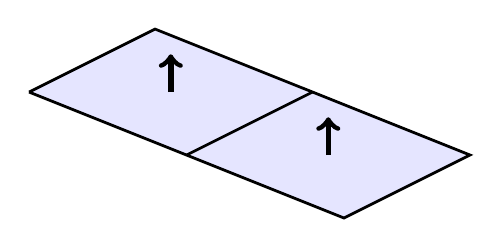
\begin{tikzpicture}[scale=4, x={(0.5cm,-0.2cm)}, y={(0.4cm,0.2cm)}, z={(0.0cm,0.6cm)}]

  %%%%%%%%%% Points pour travailler %%%%%%%%%%
 \coordinate (0) at (0,0,0);
 \coordinate (1) at (0,1,0);
 \coordinate (2) at (1,0,0);
 \coordinate (3) at (1,1,0);
 \coordinate (4) at (2,0,0);
 \coordinate (5) at (2,1,0);

 %%%%%%%%%% Layer blue color %%%%%%%%%%
 \fill [color=blue!10!white] (0) -- (1) -- (5) -- (4) -- cycle ;
 
 % Quads
 \draw [line width=1] (0) -- (4) -- (5) -- (1) -- (0) ;
 \draw [line width=1] (2) -- (3) ;

 %%%%%%%%%%% Feature edge %%%%%%%%%%%
 %\draw [line width=2, color=black] (2) -- (3) node[pos=0.6, color=black, opacity=0.7, below] {} ;

 %%%%%%%%%%% Normales %%%%%%%%%%%
 \draw[->, line width=2] (0.5,0.5,0) -- (0.5,0.5,0.2);
 \draw[->, line width=2] (1.5,0.5,0) -- (1.5,0.5,0.2);

\end{tikzpicture}
\end{document}